\chapter{Conclusion, Discussion and Future Work\label{chap:discussion}}
In this chapter I will conclude the work conducted in this paper, reflect back onto the results and suggest the next steps for the designed framework. I will also overview my achievements, slowdowns and difficulties found.

\section{Conclusion}
In this paper I have introduced a novel method of authenticating clients connecting to arbitrary MQTT Brokers through a middleware framework storing persistent information on Ethereum blockchain, allowing for higher transparency and availability. I have started by providing a motivation for the project, bringing up that standard MQTT protocol offers only limited authentication methods, with no option to log audit trails. Recent legislature requiring data administrators to adhere to specific set of rules dictating how the data should be stored, maintained and erased if requested was also discussed.

As the project was concerning a lot of sophisticated software such as MQTT or Blockchain, a thorough background chapter was included in order to allow the reader to better understand the concepts and decisions taken throughout this thesis.

\section{Discussion}

\subsection{Proof-of-Stake vs Proof-of-Authority}
When I first introduced conecpt of blockchain in this paper, I discussed the differences between proof-of-stake and proof-of-authority consensus algorithms. As a reminder, Proof-of-Stake involves mining rewards for adding new blocks to the chain (thus involves currency) and is currently used for the public Ethereum network, whereas Proof-of-Authority doesn't involve any rewards and all blocks are verified by a set of ``sealers'' whose job is to verify whether they can be processed or not.

\begin{figure}[h]
    \centering
    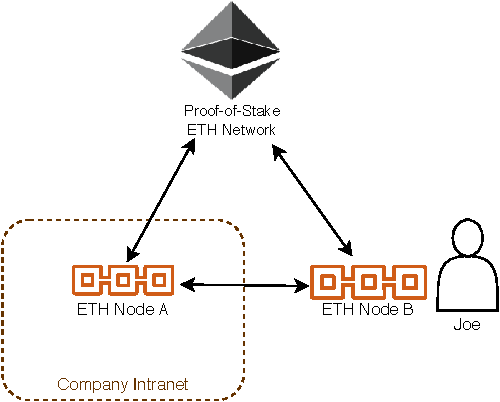
\includegraphics[width=0.7\textwidth]{blockchain_pos}
    \caption{Public Proof-of-Stake network}
    \label{fig:blockchain_pos}
\end{figure}
\begin{figure}[h]
    \centering
    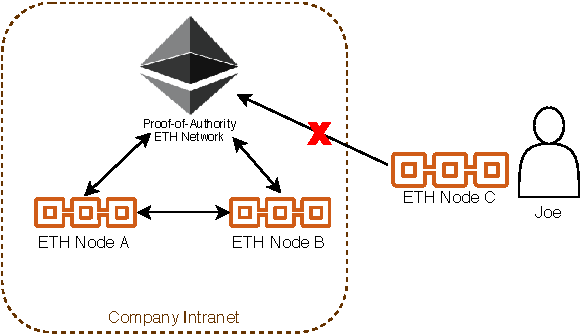
\includegraphics[width=0.7\textwidth]{blockchain_poa}
    \caption{Private Proof-of-Authority network}
    \label{fig:blockchain_poa}
\end{figure}

Figures \ref{fig:blockchain_pos} \& \ref{fig:blockchain_poa} illustrate those differences. In the first example, company has complete control over its blockchain network and nobody from the outside can read it or add new blocks. Even though Joe has configured his own node, he won't be able to connect to it. In the second example, the company is connecting to the public node, to which Joe - and anyone else - can also connect to read or submit new blocks.

Let's first look at Proof-of-Stake. This includes all benefits coming from blockchain architecture.  That is, the entire layer is decentralised, meaning that hardware failure will not cause data loss, as every participant will be holding a copy. This ensures a true 100\% uptime of data layer. Moreover, all transactions are transparent and immutable. Nobody can deny submitting it or alter the past by removing some blocks from the chain (which is not even possible to begin with) - perhaps this would be the most beneficial by authorities and law enforcement organisations, which no longer have to trust data provided by the company, as they are able to host their own node and read stored data.

\subsection{Comparison with State-of-the-Art}

\section{Reflection}

\subsection{Achievements}


\subsection{Difficulties \& lessons learnt}
When starting to plan this project at the end of the last year, I would never anticipate that I would have to conduct it in circumstances like that. I have to admit, working on my project fully remotely has been a big challenge which made me appreciate face-to-face teaching even more. As much as my online meetings were going smoothly and without problems,

As I planned my risk management when writing the project plan, I didn't take global pandemic into an account - and I don't think that anyone did. With remote work

\section{Future Work}

\subsection{Testing TLS}
Following up from the evaluation chapter, we deduced a significantly increased performance loss when proxing TLS connections from Client towards FlyTrap and then from FlyTrap to MQTT Broker. Further testing could be needed to determine whether the impact is greater on \mbox{Client<->FlyTrap} or FlyTrap<->Broker side and provide appropriate guidance on how to provide the best possible performance.

For example, for situations where both FlyTrap and MQTT Broker are located on the same network, it would be wasteful to encrypt packets flowing between FlyTrap and Broker, as man-in-the-middle attacks would not be possible, since all traffic occurs on loopback network device\footnote{Also known as localhost, i.e. inter-process communication through TCP.}. It would be interesting to see whether enabling TLS only on the first part of the journey provides any significant gains.

Furthermore, alternative methods of encrypting TCP packets should be explored. This project uses the standard TLS session with all settings left at default, so tests involving different cipher suites and different key-exchange algorithms would be beneficial.
\subsection{WebSockets}
The most recent versions of popular MQTT Brokers (such as Mosquitto) introduced support for WebSockets - with many of the testing online brokers already offering support, e.g. HiveMQ WebSocket based broker can be accessed under broker.hivemq.com:8000. WebSocket \cite{fette2011websocket} are built on top of HTTP layer, meaning that all traffic flows through a single port. No longer it is necessary to utilise multiple ports to send concurrent messages.

\begin{figure}[h]
    \centering
    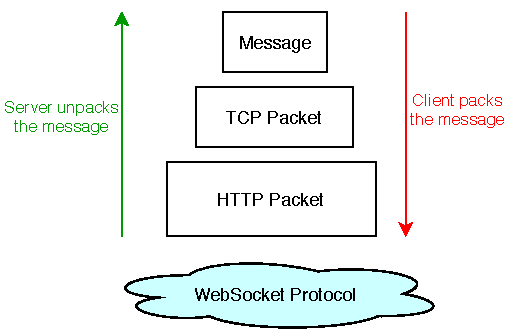
\includegraphics[width=0.7\textwidth]{websockets}
    \caption{Overview of WebSocket protocol}
    \label{fig:websockets}
\end{figure}

Figure \ref{fig:websockets} demonstrates how messages are encapsulated by the client and then unpacked by the server. The most apparent benefit is the increased number of possible proxy connections. FlyTrap currently is tied to the maximum of 65535, which is the maximum number of ports on Linux. Secondly, lot of firewalls forbid outgoing and incoming connections from non-standard ports. Whenever a new proxy connection is initiated, FlyTrap opens a new ephermal port, which could otherwise be blocked.

At the moment, the framework operates solely on TCP layer, sending raw TCP/TLS packets. By adding a support for WebSocket protocol, the limit of maximum concurrent connections could be increased and by limiting it to a singular port (for example, 80), it could become more accessible to devices behind strict firewalls.
\subsection{Device Authenticity}
FlyTrap currently relies only on authentication through a signature containing public key, signed by the corresponding private key. While it works perfectly fine for the purposes of this project and provides a reasonable protection barrier from attackers, it does not take into consideration situations where the IoT device containing the private key / signature gets stolen and its data becomes compromised. At this point, the attacker could calculate their own signatures and start making requests against FlyTrap. IoT devices are often neglected when it comes to physical security - they are often placed in public spaces, where anyone could potentially remove it. Normally, it is not a concern, as they are not targeted due to their low cost, but by placing secret data (which signature / private key could be considered as such), it might cause them to become a target.

This problem fell out of scope for this project and thus it was not considered when designing the system. To tackle this, one might want to introduce methods of verifying the authenticity of connecting devices. In 2012 Apple filed a patent with United States Patent and Trademark Office \cite{omernick2012systems} offering a solution for this problem. In the future, ideally FlyTrap should be enhanced by a similar solution, such that it would be able to identify whether the connecting device is a genuine IoT sensor or an attacker connecting from a laptop.